% % % Headers and definitions
\documentclass[11pt]{article}
%\usepackage{times}

\usepackage{fullpage} % sets more standardized margins
\usepackage{graphicx} % some graphics functions I use 
\usepackage{abstract} % abstract function
\usepackage{mathtools}
\usepackage{float}
\usepackage{array}
\usepackage{gensymb}
\usepackage{verbatim}
\usepackage[utf8]{inputenc}
\usepackage{amsmath}
\usepackage{multirow}

\usepackage[font=small]{caption}

%% latexdiff stuff
%DIF PREAMBLE EXTENSION ADDED BY LATEXDIFF
%DIF UNDERLINE PREAMBLE %DIF PREAMBLE
\RequirePackage[normalem]{ulem} %DIF PREAMBLE
\RequirePackage{color}\definecolor{RED}{rgb}{1,0,0}\definecolor{BLUE}{rgb}{0,0,1} %DIF PREAMBLE
\providecommand{\DIFadd}[1]{{\protect\color{blue}\uwave{#1}}} %DIF PREAMBLE
\providecommand{\DIFdel}[1]{{\protect\color{red}\sout{#1}}}                      %DIF PREAMBLE
%DIF SAFE PREAMBLE %DIF PREAMBLE
\providecommand{\DIFaddbegin}{} %DIF PREAMBLE
\providecommand{\DIFaddend}{} %DIF PREAMBLE
\providecommand{\DIFdelbegin}{} %DIF PREAMBLE
\providecommand{\DIFdelend}{} %DIF PREAMBLE
%DIF FLOATSAFE PREAMBLE %DIF PREAMBLE
\providecommand{\DIFaddFL}[1]{\DIFadd{#1}} %DIF PREAMBLE
\providecommand{\DIFdelFL}[1]{\DIFdel{#1}} %DIF PREAMBLE
\providecommand{\DIFaddbeginFL}{} %DIF PREAMBLE
\providecommand{\DIFaddendFL}{} %DIF PREAMBLE
\providecommand{\DIFdelbeginFL}{} %DIF PREAMBLE
\providecommand{\DIFdelendFL}{} %DIF PREAMBLE
%DIF END PREAMBLE EXTENSION ADDED BY LATEXDIFF
%%

%%%%%%%%%%%%%%%%%%%%%% BIB STUFF

%%% This block needed for IEEEtran control entry, edit actual entry in .bib file used
\makeatletter
\def\bstctlcite{\@ifnextchar[{\@bstctlcite}{\@bstctlcite[@auxout]}}
\def\@bstctlcite[#1]#2{\@bsphack
  \@for\@citeb:=#2\do{%
    \edef\@citeb{\expandafter\@firstofone\@citeb}%
    \if@filesw\immediate\write\csname #1\endcsname{\string\citation{\@citeb}}\fi}%
  \@esphack}
\makeatother
%%%%%%%%%%%%%%%%%%%

\usepackage{babel}
\iffalse
\usepackage[
    backend=biber, 
    natbib=true,
    style=numeric,
    style=ieee,            % ieee style for easy referencing
    sorting=none
]{biblatex}
\addbibresource{bib.bib}
\fi

%\addbibresource{IEEEabrv.bib}
%\addbibresource{IEEEexample.bib}

%\DefineBibliographyStrings{english}{
%  references = {Sources},
%}

\usepackage{etoolbox}
\patchcmd{\thebibliography}{\section*{\refname}}{}{}{}



%%%%%%%%%%%%%%%%%%%%%%

% Uncomment for hyperlinks
\usepackage{hyperref}
\hypersetup{
    colorlinks=false,
    linkcolor=black,
    filecolor=black,      
    urlcolor=black,
}

%%%%%%%%%%%%%%%%%%%%%%
\usepackage{listings}

\usepackage[T1]{fontenc}

\usepackage{color}
 
\definecolor{codegreen}{rgb}{0,0.6,0}
\definecolor{codegray}{rgb}{0.5,0.5,0.5}
\definecolor{codepurple}{rgb}{0.58,0,0.82}
\definecolor{backcolour}{rgb}{0.95,0.95,0.92}
 
\lstdefinestyle{mystyle}{
    backgroundcolor=\color{backcolour},   
    commentstyle=\color{codegreen},
    keywordstyle=\color{magenta},
    numberstyle=\tiny\color{codegray},
    stringstyle=\color{codepurple},
    basicstyle=\footnotesize,
    breakatwhitespace=false,         
    breaklines=true,                 
    captionpos=b,                    
    keepspaces=true,                 
    numbers=left,                    
    numbersep=5pt,                  
    showspaces=false,                
    showstringspaces=false,
    showtabs=false,                  
    tabsize=4
}
 
\lstset{style=mystyle}
\renewcommand{\lstlistingname}{Source}
\renewcommand{\lstlistlistingname}{List of \lstlistingname s}
%%%%%%%%%%%%%%%%%%%%%%

\renewcommand{\absnamepos}{flushleft} % left justifies abstract
\setlength{\absleftindent}{0pt}
\setlength{\absrightindent}{0pt}
\setlength{\absleftindent}{0pt}
\setlength{\absrightindent}{0pt}

% double or 1.5 spaced lines, 11 point Times New
%Roman for the text body, Arial of appropriate size for headings, a left margin of 1.5”, a right, top and bottom
%margin of 1”
\usepackage{geometry}
\geometry{left=1.5in,top=1in,bottom=1in}


% % %
% Set up IEEE style paragraphing
% % %
\setlength{\parskip}{1em} % The \par command now skips a line between paragraphs, eliminates warnings from using the \par or \\ commands
\setlength{\parindent}{0em} % Left justifies paragraphs after a \par command 
%\setlength{\belowcaptionskip}{-10pt} % change length below figure caption 
\renewcommand{\baselinestretch}{1.5}
\renewcommand*\thetable{\Roman{table}}
\begin{document}
\bstctlcite{IEEEexample:BSTcontrol}
% To enable subsubsubsections!!!
%%%%
%\newcommand{\subsubsubsection}[1]{\paragraph{#1}\mbox{}\\}
%\setcounter{secnumdepth}{4}
%\setcounter{tocdepth}{4}
%%%%

\setcounter{secnumdepth}{4}
\setcounter{tocdepth}{4}


%\setlength{\belowcaptionskip} -100
\pagenumbering{gobble} % Turn off page numbering for titles and tables

% Title and author

	\title{ 
	\textbf{ Robust Framework for Interfacing Devices (R.F.I.D.)}
    \\ ECE 403 Final Report
    \\ University of Maine}
	
\author{%\it{Forest LeBlanc, Computer Engineer}\\
  	    \it{Forest LeBlanc, Computer Engineer}\\
  	    \it{Dan Schlabig, Electrical and Computer Engineer}
  	                }
\date{\today}
\maketitle


% % % % % % % % % % % % % % %		
% Abstract 

\newpage
\begin{abstract}
\label{sec:1_abstract}

\pagenumbering{gobble}
\pagenumbering{roman}

R.F.I.D., a device that receives radio-frequency identification (RFID) tag data through serial communication from an external device and stores the data on an SD card, has been designed and tested. A microcontroller receives tag data from the external device through serial communication. Software features of R.F.I.D. included code to schedule inter-device data transfer and uploads, the design of a FAT filesystem library for use with the onboard SD card, and serial communication between the microcontroller and peripheral communication device. Hardware features include the interfacing of each module by use of a printed circuit board (PCB) and DC-DC conversion via a buck converter. The DC-DC converter's output voltage was measured as 3.33VDC with with a 56mVpp ripple while supplying a current of 271mA to a load. R.F.I.D. has been demonstrated to be capable of creating and writing a file on a FAT16 formatted SD Card, with received RFID tag data, date, and times written to the created file. No file handling performed by the project uses an existing FAT filesystem library. All project specifications were met or exceeded.



%All project specifications were met or exceeded.
% add results of project, and make abstract past tense


%This report describes the design, testing, and results of R.F.I.D., a system that receives radio-frequency identification (RFID) tag data through serial communication from an external device, and stores the data on an onboard SD card using a custom FAT filesystem.A microcontroller receives tag data from the external device through serial communication. Software features of R.F.I.D. include code to schedule inter-device data transfer and uploads, the design of a FAT filesystem library for use with the onboard SD card, and serial communication between the microcontroller and the peripheral communication device. Hardware features include the interfacing of each module by use of a printed circuit board (PCB) and DC-DC conversion via a buck converter. 
\end{abstract}

% % % % % % % % % % % % % % % 
% Tables of contents, figures, tables, acronyms, etc
\newpage % jumps to new page
\setlength{\parskip}{0em} % Don't skip a line between paragraphs for TOC and and lists of figures and tables

\tableofcontents

\newpage
\listoffigures

\newpage
\listoftables

\newpage 
\clearpage
\setlength{\parskip}{1em} % The \par command now skips a line between paragraphs, eliminates warnings from using the \par or \\ commands

\pagenumbering{arabic} % Turn on page numbering

% % % % % % % % % % % % % % %
% Introduction section  
\section{Introduction}
\label{sec:2_intro}
This report describes the design, testing, and operation of the Robust Framework for Interfacing Devices (R.F.I.D.), a device that receives Radio-Frequency Identification (RFID) tag IDs from an external device and stores the received tag IDs on an SD card for data storage. The device is essentially a data logger, meant to provide a way to record large volumes of scientific or medical data received from another device on an SD card. The device also logs the date and time at which tag IDs are received, storing that information alongside each corresponding tag ID. R.F.I.D. stores all data on a File Allocation Table (FAT) formatted SD card, which is inserted into the device. FAT is a common standard used for the organization of data on devices such as computers and SD cards. A FAT file format for the SD card allows for the easy retrieval of recorded data by any user, as the SD card can be ejected from the device and recognized by most modern operating systems.

% Add a couple sentences for motivation and compare with a a similar device

%The motivation for this project comes from ...
%Compare with a similar device on the market...

The motivation for R.F.I.D. is to support radio frequency based indoor localization. Applications of indoor localization include the monitoring of home-bound individuals and asset tracking in industrial settings. Similar projects lean more toward the latter category. Two examples include Radiant RFID and Gao RFID, both of which provide the hardware and software infrastructure for the tracking and cataloging of personnel and assets. These projects vary greatly according to the application. R.F.I.D. is similar in scope, but is primarily concerned with logging RFID tag data. In this way, R.F.I.D. provides a base for a larger, more complex system.

The project contract includes a brief description of the project and lists the project specifications, and is included in Appendix~\ref{sec:A_project_contract}. The contract specifies that a DC-DC converter supply 3.3V DC $\pm$ 10$\%$, with a maximum ripple of 200m$V_{pp}$ to the project, and that the converter be capable of supplying at least 200mA of current. The contract also dictates that the project must include a custom designed printed circuit board (PCB), that it must be capable of creating and writing files on a FAT file formatted SD card, that received RFID tag IDs must be stored with corresponding time and date stamps to the SD card, and that all file handling must be done without the use of a preexisting FAT file handling library.

The remaining sections of the report are outlined as follows. Section 2, provides a broad overview of the project. Section 3 provides specific details about the hardware and software developed for the project. Section 4 includes the results of the project. Section 5 concludes the report, while Section 6 includes the bibliography of outside sources used for the project and report.

%% Dan: So I've edited this section with what E Payne wanted. I am not sure if it's still subjunctive tense? 
% TODO: Still need to add motivation for project and also a similar device to compare/contrast. 

% % % % % % % % % % % % % % %
% Breakdown                           
\section{Breakdown}
\label{sec:3_breakdown}
R.F.I.D. consists of four distinct functional blocks and a block that represents the system input. All blocks, along with the system input and outputs, are shown in relation to each other in Figure~\ref{fig:functional_diagram}. This section discusses the function of each block in relation to the other blocks. It also introduces significant technical specifications with which each block is associated.

\begin{figure}[H]
    \centering
    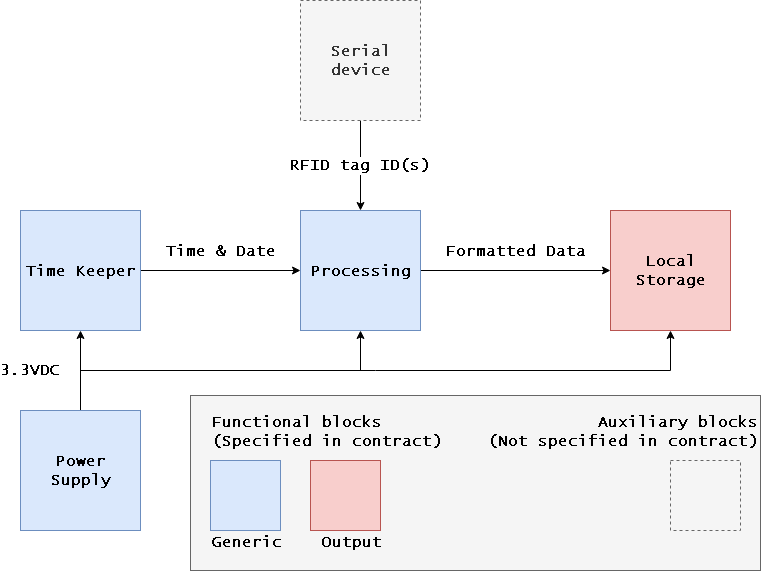
\includegraphics[width=1\textwidth]{Figures/3_breakdown/FBD.png}
    \caption{R.F.I.D. functional block diagram.}
    \label{fig:functional_diagram}
\end{figure}



R.F.I.D. receives RFID tag IDs as its system input, and outputs tag IDs, time, and date. The Power Supply block outputs a DC voltage to provide sufficient power to the Processing and Local Storage blocks. The Time Keeper block outputs time and date to the Processing block. The Processing block receives RFID tag data from an external device and outputs tag IDs, time, and date to the Local Storage block. The final system output received by the Local Storage block is stored on a FAT formatted SD card. See Appendix B for the complete schematic.

% Dan: I editted the above paragraph
% =====================================================================================

\subsection{Power Supply}

The Power Supply block consists of a battery and a DC-DC converter. The battery provides readily accessible power for the project, while the DC-DC converter regulates the battery voltage level to provide 3.3VDC $\pm$ 10\% to provide a safe voltage level to power the Processing and Local Storage blocks. That is to say, the DC-DC converter has the onboard battery as its source and the physical contents of Processing and Local Storage blocks as its load.

\subsection{Time Keeper}
The Time Keeper block consists of a quartz crystal resonator circuit and the real-time clock portion of the microcontroller used in the project. This block is required to provide the time and date information that is stipulated in the project contract. The resonator circuit provides a 32.768kHz clock frequency to the real-time clock of the microcontroller, which lowers the provided frequency to 1Hz and keeps track of both the time and date on a second by second basis. The final time and date data are passed to the Processing block, where they are used to keep track of when RFID Tag Data are received by R.F.I.D..
% Dan: I want to check on the wording of this above parag.
% =====================================================================================


\subsection{Processing}
 The Processing block receives RFID tag data via serial communication. This block receives 3.3VDC $\pm$ 10\% from the Power Supply block. The block also outputs RFID tag data, with date and time stamps, to the Local Storage block. The Processing block consists of a microcontroller. It obtains and formats all data. It also initializes all associated peripherals and general software operation of the device. This block communicates with two devices: the external device that provides the system input and the SD card where it stores data. Lastly, this block provides the memory and computational power required to write data to the Local Storage block in accordance with a FAT format.
 
 
 %Among chief concerns are the fact that several communication standards are in use by the device, requiring careful clock configuration and main program organization; and the fact that the code base must be fairly compact with room for modifications as necessary for different RFID devices or outputs.


%The Processing block consists of a microcontroller that serves two purposes. It maintains communication with an external device that provides RFID tag data, and also communicates with an SD card to record data. The microcontroller also provides the memory and computation power required to write data to the Local Storage block in keeping with a FAT format.


\subsection{Local Storage}
The Local Storage block receives RFID tag IDs, date and time stamps, from the Processing block. It is powered by the Power Supply block. Data received from the Processing block are stored on a FAT file formatted SD card. This block consists of both hardware and software; it includes a software library that controls the exchange of data to and from the SD card. However, software functions account for most of this block's complexity. The primary concern is whether the data to be read or written are formatted correctly; that is, in consistent chunks and sectors with an intact BIOS Parameter Block (BPB), which is used to glean most information about a new filesystem.

%% Dan: I'm kind of confused how to approach this subsection

% 

% % % % % % % % % % % % % % %		
\section{Details}
\label{sec:4_details}
% =====================================================================================
This section details the design of R.F.I.D. Each functional block shown in Figure~\ref{fig:functional_diagram} is analyzed separately to give a comprehensive understanding of the project as a whole. The Power Supply, Time Keeper, Processing, and Local Storage blocks are each introduced and their associated circuits or algorithms are justified. See Appendix C for a complete parts list.

\subsection{Power Supply}

The Power Supply block of R.F.I.D. powers the whole project. This block's primary purpose is to supply 3.3VDC$\pm$10\% with at least 200mA of current, and no more than 200mVpp ripple to power the STM32l476RET microcontroller and SD card of the project. A buck converter steps the main battery voltage down from a nominal 3.7V to a nominal 3.3V. 
% TODO: The above paragraph needs ore editing. I'm moving on for now

The Power Supply block consists of a buck converter circuit that regulates the input voltage from a 3.7V nominal LiPo battery. The buck converter steps the battery's 3.7V voltage down to 3.3VDC$\pm$10\% for R.F.I.D.'s microcontroller and SD card. A buck converter was chosen instead of a linear regulator because switching regulators such as buck converters are typically more energy efficient. Energy efficiency is an important consideration for battery powered devices such as R.F.I.D., since an energy efficient device will require less frequent recharging or battery replacement. The buck converter circuit is shown in Figure~\ref{fig:buck_conv_schem}.

\begin{figure}[H]
    \centering
    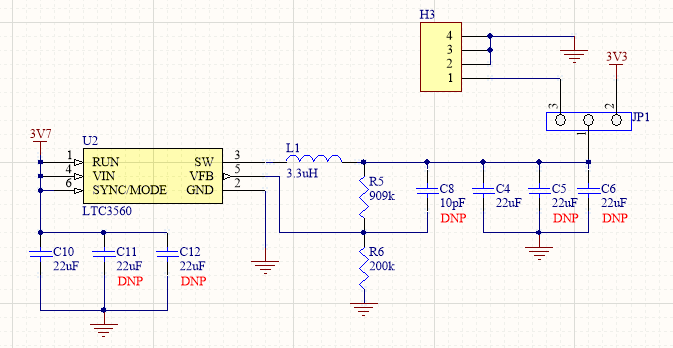
\includegraphics[width=1\textwidth]{Figures/4_details/buck_schem.PNG} 
    \caption{Buck converter circuit schematic.}
    \label{fig:buck_conv_schem}
\end{figure}

The LTC3560 buck converter integrated circuit (IC) and its associated passive components regulate the LiPo battery voltage of 3.7VDC seen at the RUN pin to 3.3VDC at pin 1 of JP1. Either pins 1 and 2 or pins 1 and 3 of JP1 can be shorted to choose the path which the 3.3VDC signal follows. With pins 1 and 2 shorted, the 3.3VDC signal powers R.F.I.D. With pins 1 and 3 of JP1 shorted, the signal is diverted to H3 so that the power supply can be tested independently of the power demands of the rest of R.F.I.D. 

The buck converter IC needs to be able to meet the demands of the Power Supply block with regards to input voltage, output voltage, and output current. It needs an input voltage range spanning from at least 3V to 4.2V t to match the range of voltages which a LiPo battery could be charged to. It also needs to have an output voltage range which includes the specified 3.3V output voltage. The IC also needs to be capable of supplying at least 200mA of current to meet contract specifications. For these reasons, the LTC3560 was thus chosen as the power supply's buck converter IC. The LTC3560 accepts an input voltage range from 2.5V to 5.5V and can output between 0.6V and 5.5V. Both the voltage provided by the LiPo battery and the specified 3.3VDC$\pm$10\% output voltage fall within these ranges, which means that the IC meets the voltage requirements of the power supply. The LTC3560 can also supply a maximum current of 800mA, which exceeds the power supply's minimum specified output current of 200mA.

%The LTC3560 was chosen because it can meet the demands of the Power Supply block with regards to input voltage, output voltage, and output current. The LTC3560 accepts an input voltage range from 2.5V to 5.5V and can output between 0.6V and 5.5V. Both the voltage provided by the LiPo battery and the specified 3.3VDC$\pm$10\% output voltage fall within these ranges, which means that the IC meets the voltage requirements of the power supply. The LTC3560 can also supply a maximum current of 800mA, which exceeds the power supply's minimum specified output current of 200mA.

L1 was chosen based upon several consideration. This inductor's saturation current rating should be above the maximum expected DC output current of the LTC3560, as the inductor would be damaged if that current is exceeded during normal operation. The inductor should also have a low estimated series resistance (ESR), so as to minimize resistive losses, as the power dissipated by the inductor would be the the current flowing through it squared times its ESR. An inductor with a large ESR would significantly reduce the buck converter's efficiency.

Inductor L1 was selected based upon both the inductor ripple current that would be seen at the SW pin of the LTC3560 and the minimum saturation current that the inductor would need. The inductor ripple current is determined by
% Inductor ripple current

\begin{equation}
\label{eq:inductor_ripple_current}
    {\Delta}I_{L} = \frac{V_{OUT}}{f\cdot L}\left(1-\frac{V_{OUT}}{V_{IN}}\right) \cite{ltc:3560},
\end{equation}

where $V_{IN}$ and $V_{OUT}$ are respectively the input and output voltages of the buck converter, while f is the switching frequency (2.25MHz) at which the IC operates, and L is the inductor value. $V_{OUT}$ is set to 3.3V while $V_{IN}$ is set to 5V to design for the worst-case input voltage, as an optional 5V USB source was initially considered for the power supply. Equation (\ref{eq:inductor_ripple_current}) is thus simplified as

\begin{equation}
\label{eq:inductor_ripple_current_simplified}
    {\Delta}I_{L} = \frac{498.6n}{L}.
\end{equation}

The minimum saturation current required from the inductor is determined by

\begin{equation}
\label{eq:inductor_saturation_current}
    I_{L,sat.} = I_{L,max} + \frac{{\Delta}I_{L}}{2} \cite{ltc:3560},
\end{equation}

where $I_{L,max}$ is the maximum DC current which can be supplied by the LTC3560's SW pin (800mA) and ${\Delta}I_{L}$ is already known dependent on the inductor value. Equation (\ref{eq:inductor_ripple_current_simplified}) and (\ref{eq:inductor_saturation_current}) are then used to compare common inductor values and their associated inductor ripple currents and minimum saturation currents, as seen in Table~\ref{tab:inductor_value}.

\begin{table}[H]
\centering
\caption{Inductor saturation and ripple currents depending on L}
\label{tab:inductor_value}
\begin{tabular}{|c|c|c|}
\hline
L (${\mu}$H) & ${\Delta}$I_L~(mA) & $I_{L,sat}~(A)$ \\ \hline
1            & 498.7         & 1.049          \\ \hline
2            & 249.3         & 0.9247         \\ \hline
2.2          & 226.7         & 0.9133         \\ \hline
3            & 166.2         & 0.8831         \\ \hline
3.3          & 151.1         & 0.8756         \\ \hline
4.2          & 118.7         & 0.8594         \\ \hline
4.7          & 106.1         & 0.8530         \\ \hline
6.8          & 73.33         & 0.8367         \\ \hline
\end{tabular}
\end{table}

The chosen inductor must have a saturation current rating of at least $I_{L,sat}$ to avoid saturating the inductor core, which would reduce the inductor's inductance below its nominal rating. The values for L and their corresponding values for $I_{L,sat}$ from Table~\ref{tab:inductor_value}, as well as having a low ESR and large saturation current, were considered while choosing the inductor.

The MAMK2520T3R3M inductor was chosen for L1. Its inductance is 3.3$\mu$H$\pm$20\% while its saturation current rating is 1.8A, well above the minimum value of 0.8756mA for an inductance of 3.3$\mu$H from Table~\ref{tab:inductor_value}. The MAMK2520T3R3M also has a low maximum ESR of 156m$\ohm$ and a saturation current rating of 1.8A, which is more than twice the maximum current that the LTC3560 IC can source. The MAMK2520T3R3M is also shielded, meaning that the magnetic flux which it produces as current flows through it is more or less contained within the inductor and consequently less likely to interfere with nearby circuit components or parts.

Next, the input and output capacitors, respectively C10 and C11, were considered. The input capacitor serves two primary purposes. It impedes the change in voltage at the input of the buck converter, essentially smoothing the voltage signal. The input capacitor also provides a low impedance path to ground for alternating current (AC) noise. This AC noise is a result of the switching off and on of the MOSFET gate inside the buck converter IC that allows inductor L1 to store and discharge energy in the form of current from its magnetic field. This AC current associated with the buck converter's duty cycle is pulled through the input capacitor via the return path provided through ground from the output of the buck converter, as well as through the battery-provided unregulated power to the input of the buck converter.

The output capacitor, like the input capacitor, serves two primary purposes. The output capacitor stores energy to meet the instantaneous current demands of the load, while the MOSFET switch inside of the LTC3560 is in its off state and no current can flow from the buck converter's input to its output. The Power Supply block should have a fast response to increased demands from its load. Otherwise, important parts of R.F.I.D. such as the microcontroller or SD card could demand more current than could be quickly supplied. Even in the MOSFET switches' on state, the delay in the propagation of power through the buck converter circuit could be too slow to meet the demands of R.F.I.D. This capacitor also smooths the output voltage of the buck converter, reducing the output Power Supply block's voltage ripple.  

ESR and equivalent series inductance (ESL) are important parameters to consider when selecting both the input and output capacitors of a buck converter. The input and output capacitors ideally have zero ESR and ESL. The larger the ESR of the capacitor, the more power is dissipated as heat and thus the less efficient that the buck converter is. A larger ESR also increases the ripple voltage seen at both the input and output of the buck converter, as the voltage across a component is proportional to both the current flowing through the component and its resistance. The ESL of a capacitor provides a parasitic inductor that will store energy as the current flowing through it varies. The energy stored in this parasitic inductor is then released when the voltage across it, the voltage ripple seen at the output or input of the buck converter, is at its peak, causing voltage and current ripples. 

The maximum RMS current allowed by the input capacitor is also important, as the capacitor will be damaged if the RMS current flowing through the capacitor is above its RMS current rating. The maximum RMS current expected to be seen at the input of the buck converter is  

\begin{equation}
\label{eq:rms_max}
    I_{RMS,max} = \frac{I_{OUT,max}[V_{OUT}\left(V_{IN}-V_{OUT}\right)]^{1/2}}{V_{IN}} \cite{ltc:3560},
\end{equation}

where $V_{OUT}$ is the output voltage, $V_{IN}$ is the input voltage, and $I_{OUT,max}$ is the maximum output current expected to be sourced by the buck converter. Setting $V_{OUT}$ equal to 3.3V, $V_{IN}$ equal to 5V, and $I_{OUT,max}$ to 800mA results in an $I_{RMS,max}$ of 379mA. 

The output voltage ripple must, as required by contract, be less than 200mVpp. This voltage can be calculated via 
%The buck converter's output voltage ripple is determined by
\begin{equation}
\label{eq:output_voltage_ripple}
    {\Delta}V_{OUT} = {\Delta}I_{L}\left(ESR + \frac{1}{8\cdot f \cdot C_{OUT}} \right) \cite{ltc:3560},
\end{equation}

where the referenced ESR is that of the buck converter's output capacitor, and f is the buck converter's 2.25MHz switching frequency. Equation \ref{eq:output_voltage_ripple} was calculated for each capacitor considered. For simplicity, the input and output capacitors were chosen to be the same.

% Capacitor is wrong, double check, looks like actually using the 1276-1771-1-ND (CL31A226MQHNNNE)
Finally, the 22$\mu$F$\pm$20\% Samsung CL21A226MQCLRNC ceramic capacitor was chosen for C4 and C10. This capacitor has a low ESR of 9m$\ohm$ at 100kHz and an RMS current rating above 379mA. The effective capacitance is reduced by 50\% to 11$\mu{F}$ due to 3.3V bias voltage at the buck converter's output. After taking this into account, ${\Delta}V_{OUT}$ is calculated via \ref{eq:output_voltage_ripple} as 5.62mVpp. Considering other parasitic resistances, such as from PCB traces, would bring the output voltage ripple closer to a more likely value, but with a margin of allowable error greater than 150mVpp between the calculated and actual output voltage ripple, the 1276-1771-1-ND is a suitable selection for C10 and C4. 
% TODO: EPayne said she couldn't follow this parag. above...Look at later

%The capacitors C5, C6, C11, and C12, labelled with do not populate (DNP) in Figure~\ref{fig:buck_conv_schem} are extra capacitors that can be placed so as to reduce the resistance of the 

The last components to choose for the buck converter circuit are R5 and R6. The values of these resistors are selected to program, or set, the output voltage of the buck converter. The LTC3560 samples, or senses, the output voltage at any given time via its $V_{FB}$ pin and compares the output voltage with a 0.6V reference voltage, located within the IC, between the $V_{FB}$ pin and ground. An internal feedback loop inside of the IC uses the difference between these two voltages to determine the duty cycle of the IC's switching on and off, which is proportional to the the IC's step-down ratio. The step-down ratio is proportional to the buck converter's output voltage divided by its input voltage. Thus, the buck converter's output voltage can be chosen by selecting values for R5 and R6.

% within 2% according to the LTc3560's datasheet

The buck converter's output voltage is
\begin{equation}
\label{eq:DC_output_voltage}
    V_{OUT} = 0.6\left(1+\frac{R_{5}}{R_{6}}\right) \cite{ltc:3560},
\end{equation}

with the 0.6V constant voltage due to the mentioned reference voltage between the $V_{FB}$ pin and ground. Solving (\ref{eq:DC_output_voltage}) for R5 given an output voltage of 3.3V shows that R5 is required to be 4.5 times R6 for the output voltage to be 3.3V. Setting R5 equal to 900k$\ohm$ and R6 to 200k$\ohm$. satisfies this requirement. The 909k$\ohm\pm$0.5\% RC0805FR-07909KL resistor and the 200k$\ohm\pm$1\% AC0805FR-07200KL resistor were then respectively chosen for R5 and R6.

% mention that 909k was chosen because very few 900k resistors available commercially, must not be a standard value. Add the calculated output voltage (is a little different from 3.3V, still far within spec)

% =====================================================================================

\subsection{Time Keeper}
\label{ss:timekeeper}

The Time Keeper block is responsible for recording the passage of time so that R.F.I.D. can write a time and date stamp for each RFID tag that it logs on the project's SD card. These time and date stamps are required by the project contract. The time stamp should be human-readable, represented in terms of hours, minutes, and seconds, instead of only elapsed seconds. Ideally, the solution for recording time and date stamps is low powered and inexpensive. R.F.I.D. accomplishes these criteria by using the hardware real-time clock (RTC) that is included as a feature of the STM32L476RET microcontroller used for the project. The RTC feature is a significant reason for choosing this microcontroller for the project. 
%  overview
% topic sentence

%The real-time clock provides accurate time and date stamps at each point of data exchange.
% problems trying to solve?:
A real-time clock is a clock used by a computer or microcontroller to record the passage of time and dates in a human-readable format. In most digital watches, computers and similar devices, a real-time clock (RTC) is used to keep track of the passage of time. An RTC or similar timekeeping device is necessary if the device needs to perform scheduled tasks on time, or to provide accurate metadata.

% What are the criteria for a solution?
% hard, firm, soft realtime
Any time a real-time clock is in use, the system in which it is a component may be characterized as one of three cases; these are "hard" real-time, "firm" real-time, and "soft" real-time systems. They can be described loosely by the effect of a scheduled signal arriving late. A "hard" system would fail catastrophically, often with bodily harm as a result; for instance, retrograde thrusters on a moon lander. A "firm" system would have its output rendered useless, but could keep functioning; an example is a Morse code device. A "soft" system is mostly unaffected and can keep operating with a tolerable amount of error. R.F.I.D. is a "soft" system; data may still be collected and stored if the timing is slightly off. Consequences of this fact are outlined below.
\par


% accuracy of calibration
An RTC can be accurate in measuring elapsed time in measuring elapsed time, referencing the time of day in a human-readable format can be complicated. Even though some devices operate their clocks from individual power sources, interruptions may still occur. Solutions often involve polling the internet to double-check the stored time. However, because there is no degree of RTC accuracy specified for this project, and because device operation is not supported without power or in low power modes, a time and date may be provided at the time of programming. The simplest solution is to use the \_\_TIME\_\_ and \_\_DATE\_\_ constants, which are defined as per C standard by the pre-processor used by the host computer. These string constants are converted into the desired numerical format, after which the real-time clock may be appropriately calibrated and managed by use of an associated Hardware Abstraction Layer (HAL) library.
\par

The RTC for the STM32l476 microcontroller requires a low speed external (LSE) oscillator. This is a crystal oscillator which can be used by the microcontroller to provide a consistent frequency. This frequency can then be divided to lower frequencies, such as 1Hz to measure the passage of time on a second-by-second basis. The microcontroller requires a clock frequency of 32.768kHz. The crystal used, X1 in the complete schematic shown in Appendix B, is the ECS-.327-CDX-1128. This crystal provides the correct clock frequency of 32.768kHZ required for the microcontroller's RTC feature to work.

% clock drift handling
Over a period of extended use, a phenomenon called clock drift is common. The crystal may oscillate at a slightly different frequency than normally specified. This may be due to environmental factors or physical defects. This is a normal process and is in fact often used in computers to provide random number generator (RNG) seeds, or pseudo-random starting values. In cases such as these, or when an application is extremely time-sensitive, clock drift is often calculated with the use of a secondary RTC.

% =====================================================================================
\subsection{Processing}
This section describes the design and application of the software algorithms that R.F.I.D. uses. These include the control of input and output serial data, management of local storage via a FAT16 filesystem, and general operation. These algorithms relate to the operation of communication protocols to either receiving and transmitting data or the processing of that data.

%The software component pertaining to parsing output of the Time Keeper block was instead described in ~\ref{ss:timekeeper} to avoid confusion. 

\label{sss:FAT}
\subsubsection{FAT Filesystem} % How the data exchange actually happens

%NEEDS AN INTRO FOR SUBSUBSECTION HERE
R.F.I.D. needs to be able to be able to write formatted tag data with time and date stamps to a FAT formatted SD card. To accomplish this, it must be capable of communicating with an SD card via a digital communication protocol. R.F.I.D. must also be able to format data appropriately for the FAT filesystem present on the SD card. Otherwise, any written or logged data, as the project's final output, would not be readable. extensive software is required to conform to the requirements of writing to and reading from a FAT filesystem. There are also different variations of FAT filesystems that R.F.I.D. could support. 


% background info
%The File Allocation Table (FAT) is a type of filesystem where a table is used to describe the location 

%A File Allocation Table (FAT) filesystem  memory is segmented by clusters, which are contiguous blocks of memory.
%Files and directories (or "folders") are stored as directory entries that may occupy one or more clusters.
%Clusters may further be divided into sectors, which rarely hold any special significance. One exception is the boot sector, which contains vital information about the corresponding filesystem. Specifically, most of this useful information is contained within the BIOS Parameter Block (BPB), which is the first section of memory to be read by any device. 
%A
%\par
%to organize files contained in a data storage device, such as a USB drive or SD card. 

\label{ssss:FAT_background}
\textbf{Background of the FAT Filesystem:} A File Allocation Table (FAT) filesystem is a type of filesystem that uses a table, or index, called the FAT to mark the location of different chunks of memory. R.F.I.D. must be able to create files and log data on a FAT formatted SD card, without using an existing library. Consequently, a huge portion of the software developed for R.F.I.D. relates to adhering to a FAT standard. Thus, a description, or background, of FAT filesystems is required.

%Consequently, a huge portion of the software developed for R.F.I.D. relates to FAT16, the type of FAT filesystem that the project interfaces with. Thus, a description, or background, of FAT16 is required.
 
A FAT volume is divided into four regions. These regions are the reserved region, the FAT, the directory table, and the data region. Figure~\ref{fig:FAT_regions} shows, from top to bottom, the first memory region to the last.

\begin{figure}[H]
    \centering
    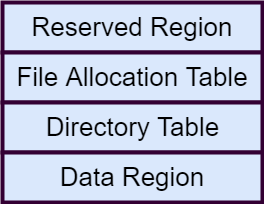
\includegraphics[width=0.5\textwidth]{Figures/4_details/fat_regions.png} 
    \caption{A FAT volume's four regions.}
    \label{fig:FAT_regions}
\end{figure}

Each region is further divided into sectors. All sectors on a FAT volume are the same size in bytes. The data region's sectors are also organized into clusters, with each cluster containing a fixed amount of sectors. The data region contains the contents of each file. Each file is allocated a number of clusters depending on its size. The directory table is where files are listed in separate entries. Each file entry contains information including the file's name, its size in bytes, and which cluster the file's data begins in. 

The FAT is a table of all clusters that are allocated for files. Each entry in the FAT has a value. This value may be 0x00 if a cluster is not yet allocated for a specific file, the number of the next cluster allocated for the file, or 0xFF if that cluster is the last one containing the file's data. The reserved region's first sector is the boot sector. The boot sector contains vital information about the filesystem that is needed to calculate the size and location of each region.

%Each cluster is represented by a 16-bit entry in the table, which is how FAT16 gets its name.

%An operating system will read the boot sector to determine how to traverse a FAT volume. It then will read the directory table to know which files are in the volume. To access a specific file for reading or writing, An operating system will go to the start cluster in the data region that is noted in the file's directory entry. If the operating system needs to access more data clusters, it will follow the allocated clusters for the file, like a linked list, by viewing the FAT. 


% different FAT versions
\textbf{Design Considerations:} FAT in fact accounts for a family of related filesystem standards, and so the necessity arises to choose which variant or variants to support. Options include FAT12, FAT16, and FAT32. Other derivations exist but are generally far more complex than needed for the scope of this project.
The chief difference between these three is the size of their cluster addresses. FAT12 uses a 12-bit address, FAT16 a 16-bit address and FAT32 a 32-bit address. A larger address entails the availability of more clusters, but also universally increased complexity.
%why?
\par

% size constraints
One key limiting factor to consider when developing this library is that of size. Each FAT variant has both a minimum and maximum available size. The minimum size for any variant is far less than even 1GB, and so can be neglected. The micro-SD cards most readily available to the design team are 4GB in nominal size, thus it's preferable to use a FAT variant that can work with a 4GB SD card without having to partition it. Table~\ref{table_fatsize} shows that either FAT16 or FAT32 would be sufficient, supporting a 4GB volume size~\cite{src_FAT-filesizes}.

%table of max volume sizes
\begin{table}[H]
\centering
\caption{Maximum volume sizes supported by FAT12, FAT16, FAT32.}

\resizebox{1\textwidth}{!}{%
\begin{tabular}{|l|l|l|}
\hline
\textbf{FAT variant} & \textbf{\begin{tabular}[c]{@{}l@{}}Approx. maximum volume size\\w/ 128 sectors/cluster\end{tabular}} & \textbf{\begin{tabular}[c]{@{}l@{}}Maximum volume size\\w/ 128 sectors/cluster\\ \\ (in bytes)\end{tabular}} \\ \hline
FAT12 & 255 MB & 267,694,024 \\ \hline
FAT16 & 4095 MB & 4,294,180,864 \\ \hline
FAT32 & 2047 GB & 2,198,754,099,200 \\ \hline
\end{tabular}%
}

\label{table_fatsize}
\end{table}

% \cite{src_FAT-filesizes}

The choice of FAT16 would meet the needs described, and is less difficult to implement than FAT32. As such, FAT16 was chosen as the sole supported FAT archetype. 

Features included in many FAT libraries are not required for the purposes of R.F.I.D. These include the ability to create and traverse sub directories, create files with `long' names, and handle file permissions. As such, the FAT16 library developed for R.F.I.D. features a basic set of core functions.

Figure~\ref{fig:FAT_layers} shows a model of the structure of a FAT filesystem and a corresponding library, modified in this case to include only the components essential to the operation of R.F.I.D.

\begin{figure}[H]
    \centering
    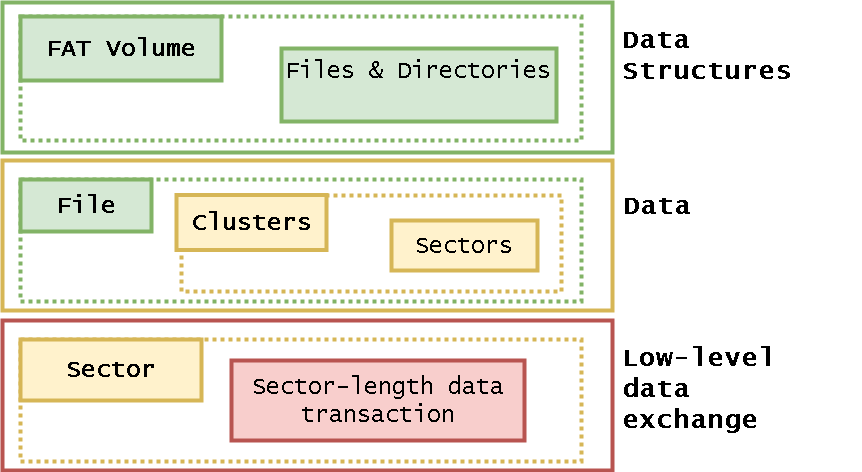
\includegraphics[width=1\textwidth]{Figures/4_details/FAT_layers.png} 
    \caption{Hierarchy of FAT library and associated data.}
    \label{fig:FAT_layers}
\end{figure}

\label{ssss:FAT_design}
\textbf{FAT16 Library Design:}
Three routines that make up the majority of the developed FAT16 library are used to navigate and modify the SD card's FAT16 volume. Each of these routines either initializes the files system, creates a file, or writes to a file. The initialization routine accepts a pointer to a struct that represents a FAT16 filesystem. It reads the boot sector on the SD Card to retrieve important values like the number of bytes per sector, number of sectors per cluster, and the total number of sectors on the volume The routine uses these and other parameters in the boot sector to calculate further information, such as each region's starting sector and size in sectors. These retrieved and calculated values are then stored in the filesystem struct for later use by the file creation and write routines.

The file creation routine initializes the contents of a struct that represents the file which data will be written to. It also initializes this abstracted file on the SD card's physical FAT16 volume. This routine reads the directory table's first sector into a buffer, which it then modifies to add an entry for the file to be created. This entry includes the name of the file, the size of the file in bytes, and the file's starting cluster. While there are additional attributes that a file entry may have, these three constitute the minimum required for a directory entry to be correctly read by an operating system. The file name is always "DATA.TXT," as R.F.I.D. only needs one file to write tag IDs and time data to. The start cluster is, for the same reason, always the same. The file size is set to zero, as a newly created file will begin with no data. The routine concludes its initialization of the file's directory entry by writing the modified buffer back to the FAT16 volume and storing the file attributes in the file entry struct so that the write routine can retrieve and update information it needs about the file.

The file creation routine then updates the filesystem's FAT to contain an entry for the file's starting cluster. This cluster is marked with 0xFF to signify that no further clusters are allocated for the file. The routine initializes a buffer for the FAT's first sector and writes it to the SD card. At this point, DATA.TXT can be viewed as an empty file by an operating system that supports FAT16.

The write routine receives a pointer to a buffer containing data to write to the file's allocated data clusters. It also receives pointers to the structs representing the filesystem and file to write to, as well as the amount of data, in bytes, to write to the file. This routine reads the file's end sector into a buffer that it appends data to so that the current sector, which may contain already written data, is not overwritten. The routine appends data in the buffer until all received data has been stored or the buffer is filled with one sector worth of data. At this point, the routine writes the modified buffer to the SD card. The routine will continue to iterate the current data cluster by one until all data has been written to the SD card or the first sector in the FAT has been completely filled with entries for the file, as this routine does not support a FAT that occupies more than one sector. Before the write routine exits, it writes FAT entries to allocate any new clusters required to contain the file's data. 





    % initialize the filesystem: 
    %  -read SD card's boot sector
    %  - put important values (bytes per sector, sectors per cluster, )
    % - calculate which sector each region starts in
    % - 
    % create the file:
    % - allocate buffers for two sectors, one in the directory table and another in the FAT
    % - set important file attributes in file struct, like start cluster, end cluster, file size (init to 0) file name
    % - Put values for the file's directory entry in the directory table, write the buffer to the SD Card
    % - mark the file's start cluster with 0xFF in FAT because the file is only allocated one cluster to begin 
    % - Write to the FAT buffer, write the FAT buffer to the first sector of the FAT
    
    % write to the file: (This one is a doozy)
    % - The write routine is called each time data needs to be written to a file
    % - Receives pointers to to the filesystem struct, the struct for the file to write to, the buffer containing data to write, and an integer for the number of bytes to write.
    
    % - Fills data into a sector-sized buffer until all the data to write is in the buffer or the buffer has has enough data to fill the current sector
    % - Writes the buffer to the file's current data sector
    % - iterates the current sector in file struct if the sector has been filled
    % - Also checks if the current cluster is filled, iterates the current cluster in file struct if so
    % - Continues this process until there are no more bytes left to write
    % - Allocates a new cluster in the FAT if a new cluster has been written to
    % updates the file size by the amount of bytes written before finally leaving the routine.


\label{ssss:FAT_application}
\textbf{Application of the FAT16 Library:} The operation of the library has so far been described without detailing the routines used to actually exchange data. These routines operate on a lower level, closer to the operation of physical hardware.  The abstraction of a FAT library must correspond to physical read/write operations. Figure~\ref{fig:FAT_readwrite} shows a brief overview of the four `steps' associated with any such data transaction. 

\begin{figure}[H]
    \centering
    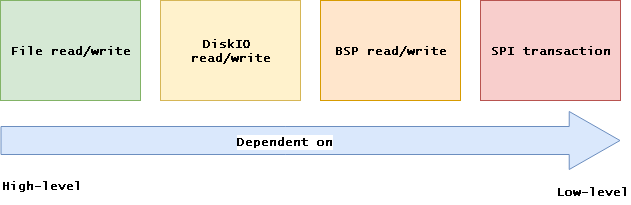
\includegraphics[width=1\textwidth]{Figures/4_details/FAT-RWflow.png} 
    \caption{Order of occurrence for read/write routines.}
    \label{fig:FAT_readwrite}
\end{figure}

At the lowest level of digital logic, each data transaction is made via serial peripheral interface (SPI), a common serial communication standard. A board support package (BSP) is re-purposed from a commercial device similar in function to R.F.I.D., and coordinates these transactions. The BSP initializes and configures the microcontroller's SPI ports, handling of errors, and formatting of all data transfers. The BSP connects to the FAT library through the diskIO layer, which is essentially an intermediate step that segments data sector-by-sector and specifies the external mechanism by which to read and write data -- in this case, of course, the BSP. All diskIO functions are called by the basic read and write functions that reside in the highest level of the FAT library. These are the functions that will in turn be called directly by the main program.
% above paragraph needs some work

Whenever an electronic storage device, such as an SD card, is used, it is good practice to use an `eject' feature. This feature notifies the device, in this case the microcontroller, to finish writing to or reading from the SD card and to notify the user once the SD card may be removed. R.F.I.D. features a simple combination of an `eject' button and notification LED. An external interrupt is generated when the button is pressed, setting a flag that the user has opted to cease the logging of data and to eject the card. If a write routine is in progress, it will conclude and no more write or read routines will begin. Then, the notification LED is turned on to alert the user that the SD card can be safely removed without damaging it or corrupting its FAT16 filesystem.

% TODO
\subsubsection{General Microcontroller Operation}
% usart in uart out
\textbf{Choice of microcontroller:} R.F.I.D. uses the STM32l476RET6 microcontroller because it easily meets all design criteria. Most importantly, it features 512KB of flash memory, ample for the operation of a potentially large FAT library, and it is commonly used for similar FAT-based file storage applications. The device also has 64 pins, enough to support all peripherals in use with some moderate overhead for future modification. Lastly, the team was more familiar with the STM32 family of microcontroller than any alternatives.

\textbf{Communication:} The software component of R.F.I.D. is also responsible for interfacing with connected devices. The input device is described as an RFID tag reader in Section~\ref{sec:2_intro}. The presence of such a reader is not vital to the operation of R.F.I.D.; as such, it may be simulated. A Raspberry Pi 3B serves this purpose whenever possible. It supplies 24-character RFID tags that may be either randomly generated or defined in a separate list. These tags may be transmitted at random or defined intervals of time to mimic the operation of a functional RFID reader. This connection takes place over the Universal Asynchronous Receive/Transmit (UART) serial bus, as many RFID tag readers feature the same bus.

On the microcontroller end of the connection, data is accepted over UART via the Direct Memory Access (DMA) controller. DMA is simply a module included in the STM32 standard that allows safe transfer of information between devices in a way that does not interfere with program operation or shared resources. This feature is not strictly necessary for R.F.I.D. in its current state, but is worth including in the case that more devices were to be connected. 

The project also has a USART connection available so that useful debugging information can be obtained. A USART is similar to UART but may operate synchronously, meaning information can be sent and received at the same time. This bus displays information about the program status, success or failure of subroutines, and useful variables, to varying degrees of detail as specified by the user. The output would most commonly be a personal computer, because a USART-to-USB adapter simplifies the connection. For more rigorous debugging, the USART transaction may even be intercepted and interpreted by the host computer before being sent.




% % % % % % % % % % % % % % %		
% Results                           
\section{Results}
\label{sec:5_results}
% forecast
    % overall performance
    This section details the observable performance of R.F.I.D. following its design, assembly and testing.
    Of the highest concern is the performance of the power supply functional block because it corresponds to the only quantitative specification. As such, this section will describe the power supply block first.
    Because the Local Storage and Time Keeper functional blocks share three technical specifications, they have been grouped together.
    The printed circuit board will be discussed lastly for a very brief description of its functioning.

\subsection{Power Supply}
% RELEVANT SPECS:
% DC-DC converter supplies 3.3V DC ±10% with a maximum ripple of 200mVpp and capable of at least 200mA
The specifications for the power supply were tested by quantitative measurements.  Prior to measuring for specifications, the output of the buck converter circuit was bypassed to H3 by placing a SPC02SYAN jumper between pins 1 and 4 of JP1, so as to test the Power Supply block independently from the rest of R.F.I.D. A ROX3SJ12R resistor with a nominal resistance of 12$\ohm{\pm}$5\% and a power rating of 3W was also placed between pins 1 and 4 of H3 to act as a test load between the output of the buck converter and ground. This test load was measured at 12.3$\ohm$ prior to its placement. All DC measurements were performed with a CSI2010 multimeter, while AC measurements were performed with a Tektronix MSO2014 oscilloscope paired with PVP2150 passive oscilloscope probes set to 10x attenuation.

First, the power supply's DC output voltage and output current capability were tested. An Adafruit 2011 battery was inserted into battery connector CON1 to supply a 3.7VDC source to the input of the buck converter circuit. The buck converter's DC output voltage was then measured across the test load as 3.33VDC, which is 0.9\% greater than 3.3VDC, and well within the allowed 3.3VDC$\pm$10\%. With a 3.3VDC output voltage, and a resistance of 12.3$\ohm$, the output current was calculated via Ohm's law as 271mA, which meets and exceeds the specification for the power supply's output current capability. At this point, only the output voltage ripple was left for the measurement and verification of the project's power supply specifications.

%he DC and AC components of the buck converter's output voltage were measured separately by placing a test load between 

Next, the output voltage ripple was tested via an AC voltage measurement across the test load, with the same setup as used for prior measurements. The oscilloscope probes, while connected to channel one of the oscilloscope, were placed between the buck converter's output and ground, with the test load still in place. Since only the AC component, or ripple, of the output voltage was being measured, the oscilloscope was set to AC coupling to block the DC component of the voltage being measured. Since this step eliminated the DC voltage from the measurement, the y-axis scale could be decreased so as to obtain a visible and accurate measurement of the voltage ripple. The oscilloscopes horizontal scale was then set to 400$\mu$s per division, while the vertical scale was set to 0.05 per division. The measured ripple voltage is shown in Figure~\ref{fig:voltage_ripple}.

\begin{figure}[H]
    \centering
    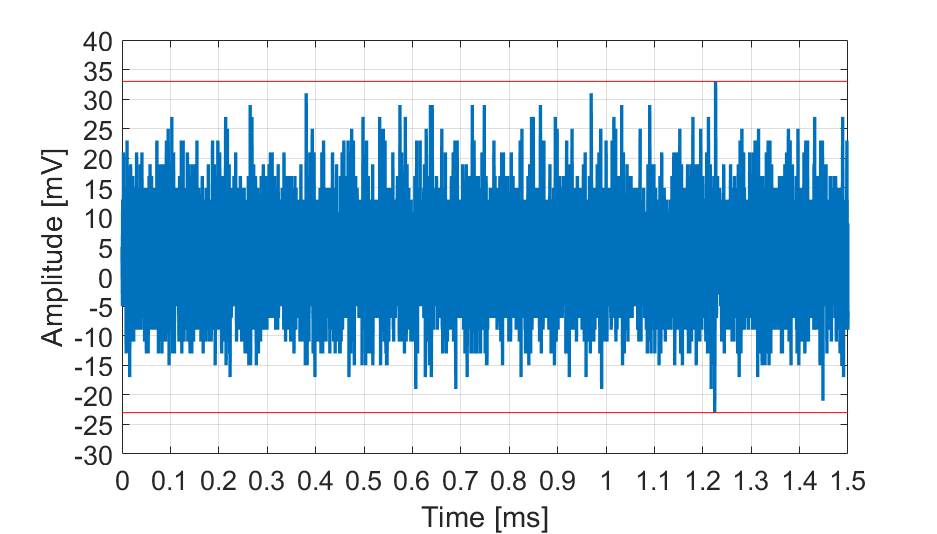
\includegraphics[width=1\textwidth]{Figures/5_results/supply1_polished_draft.png} 
    \caption{Power supply AC output voltage.}
    \label{fig:voltage_ripple}
\end{figure}

Each horizontal red line shows where the measured voltage is at its maximum or minimum value. The maximum voltage is at 33mV, while the minimum voltage is -23mV. The peak to peak ripple of the power supply's output voltage is found by taking the difference between these minimum and maximum voltages. The power supply's output voltage ripple is thus 56mV, which is 144mV below the maximum allowed by specifications. The power supply meets the specification for an output voltage ripple of less than 200mVpp.


\subsection{Processing and Time Keeper}
% RELEVANT SPECS:
% Capable of creating and writing files on a FAT formatted SD card for data storage
% Received RFID tag ID, date, and time written to file
% File handling done without using an existing FAT file system library

% methodology
% visual inspection
% Autopsy? HxD editor?
% compare log of sent data to log of received data
The Processing functional block corresponds to three purely qualitative contract specifications, making discussion somewhat difficult. Essentially, this block, and R.F.I.D. as a project, can successfully log tag data, with corresponding date and time stamps, to file on a FAT16 formatted SD card. All file handling, including the creation of files, and writing to files is done with a custom FAT file handling library.
%All file handling; including creation and writing, using a FAT library and its associated data structures; takes place without issue.

The data storage was tested by placing a FAT16 formatted micro SD card with no files on it inside P1, R.F.I.D.'s SD card holder. R.F.I.D. was then turned on by supplying power to the PCB via a 3.7V LiPo battery. R.F.I.D. then created a .txt file on the SD card via SPI with a set number of RFID tag IDs with corresponding time and date stamps. Once R.F.I.D. had closed the created file, which was noted by running the application code through a debugger mode during testing, the SD card was then removed from P1.

The SD card was then attached to a personal computer, and its contents were examined using a file explorer to open the SD card like a folder. If the file was not created according to the FAT16 standard, the personal computer would show the folder as being empty. The previously non-existent file was seen in the SD card contents, confirming that R.F.I.D. could create a file on a FAT formatted SD card. 

Next, the text file was opened on the personal computer. The contents of the created file contained the RFID tag IDs with their corresponding times and dates. This test confirmed the specification for creating and writing files on a FAT formated SD card for the storage of RFID tag IDs, date, and time. 

For additional confirmation, the forensic filesystem analysis software "Autopsy" was employed to confirm that none of the created files had been altered or tampered with \cite{src_autopsy}. This software can be used to show a hex dump, which shows the SD card's memory, and thus the FAT16 filesystem, as a sequence of hexadecimal numbers. This software package, and packages like it, were integral to develop, test, and verify the correct creation of FAT16 files. A view of the raw filesystem contents is shown in Figure~\ref{fig:notamper}. 


%%%%%%%%%%%%%%%%%%%%%%%%%%

% can be used if needed to reach page limit


\begin{figure}[H]
    \centering
    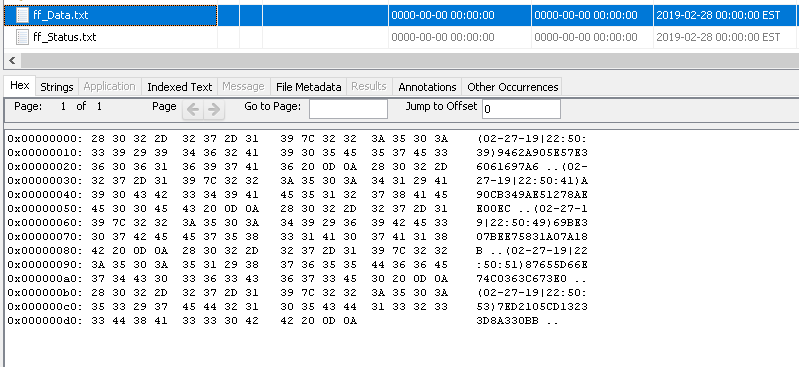
\includegraphics[width=1\textwidth]{Figures/5_results/SD_notamper.png} 
    \caption{Hex readout and excerpt of file metadata.}
    \label{fig:notamper}
\end{figure}

A quick indicator is the lack of corresponding timestamps, showing that a particular file has been edited only by a FAT library without timestamping features, as is the case for R.F.I.D. As the library used for FAT file handling was created by the design team, this specification has been met. All specifications related to the storage of data and FAT file handling have been met.

%%%%%%%%%%%%%%%%%%%%%%%%%%

\subsection{PCB}
% RELEVANT SPECS: 
% Uses a custom printed circuit board (PCB) 

All components of R.F.I.D. are located on a 4-layer PCB. This PCB was designed using the Altium design software. Next, the design was sent to JLCPCB for manufacturing. A mix of both custom-made and generic PCB footprints were used in the design of the PCB. The dimensions of the designed PCB are 61x89mm, and the thickness of the board is 1.6mm. The PCB layout as viewed from its component side is shown in Figure~\ref{fig:pcb}.

\begin{figure}[H]
    \centering
    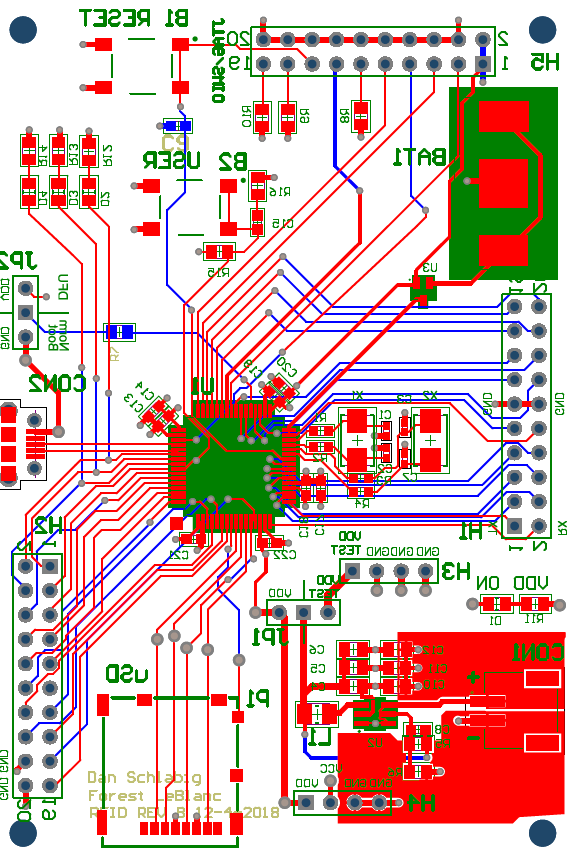
\includegraphics[scale=0.7,angle=90]{Figures/5_results/pcb_printout_3_1,2019_roughdraft.PNG} 
    \caption{PCB layout viewed from the component side.}
    \label{fig:pcb}
\end{figure}

% this part needs to be after the figure
Blue lines show traces on the bottom side of the board, while red lines show traces on the component side of the board. Four mounting holes are located on each corner of the PCB so that the PCB can be safely mounted above whatever surface that it is placed on. The project uses a custom PCB designed by the creators of R.F.I.D. Thus, the project specification for using a custom PCB is met.

% % % % % % % % % % % % % % %		
% Conclusion                                                
\section{Conclusion}
\label{sec:6_conclusion}
\iffalse
ABSTRACT:


The proposed work is a system to  receive  radio-frequency identification (RFID) tag data through serial communication from an external device, and to save the data on an onboard SD card using a custom FAT filesystem.  The RFID tag data may be simulated with no physical significance.
A microcontroller receives tag data from the external device through a wired communication bus. Software features of the proposed work include code to schedule inter-device data transfer and uploads, the design of a FAT filesystem library for use with the onboard SD card, and serial communication between the microcontroller and the peripheral communication device(s). Hardware features include the interfacing of each module by use of a printed circuit board (PCB) and DC-DC conversion.


\fi
This report has described the theory, design and function underlying R.F.I.D.
The project was found to satisfy its requirements in receiving and logging RFID tag data with associated date and time stamps on a FAT formatted SD card. The device is operational on a custom PCB, and all communication and power regulation occurs as desired. The project's 
The project's custom FAT filesystem library, however, is not operational. As such, the associated specification has not been met, leaving four of five specifications satisfied.

R.F.I.D., a device that receives radio-frequency identification (RFID) tag data through serial communication from an external device and stores the data on an SD card, has been designed and tested. A microcontroller \DIFdelbegin \DIFdel{received }\DIFdelend \DIFaddbegin \DIFadd{receives }\DIFaddend tag data from the external device through serial communication. Software features of R.F.I.D. included code to schedule inter-device data transfer and uploads, the design of a FAT filesystem library \DIFdelbegin \DIFdel{library }\DIFdelend for use with the onboard SD card, and serial communication between the microcontroller and peripheral communication device. Hardware features \DIFdelbegin \DIFdel{included }\DIFdelend \DIFaddbegin \DIFadd{include }\DIFaddend the interfacing of each module by use of a printed circuit board (PCB) and DC-DC conversion via a buck converter. The DC-DC converter's output voltage was measured as 3.33VDC with with a 56mVpp ripple while supplying a current of 271mA to a load. R.F.I.D. has been demonstrated to be capable of creating and writing a file on a FAT16 formatted SD Card, with received RFID tag data, date\DIFaddbegin \DIFadd{, }\DIFaddend and times written to the created file. \DIFdelbegin \DIFdel{All }\DIFdelend \DIFaddbegin \DIFadd{No }\DIFaddend file handling performed by the project \DIFdelbegin \DIFdel{did not use }\DIFdelend \DIFaddbegin \DIFadd{uses }\DIFaddend an existing FAT filesystem library. All project specifications were met or exceeded.



%All project specifications were met or exceeded.
% add results of project, and make abstract past tense


%This report describes the design, testing, and results of R.F.I.D., a system that receives radio-frequency identification (RFID) tag data through serial communication from an external device, and stores the data on an onboard SD card using a custom FAT filesystem.A microcontroller receives tag data from the external device through serial communication. Software features of R.F.I.D. include code to schedule inter-device data transfer and uploads, the design of a FAT filesystem library for use with the onboard SD card, and serial communication between the microcontroller and the peripheral communication device. Hardware features include the interfacing of each module by use of a printed circuit board (PCB) and DC-DC conversion via a buck converter. 
% % % % % % % % % % % % % % %
% % % % % % % % % % % % % % %		
% Appendices


\renewcommand*{\UrlFont}{\rmfamily}



%\newpage
\nocite{*}

%\label{sec:references}
%\printbibliography[heading=none]
%\renewcommand\refname{}
\section{References}
%% APPENDICES
%\endpage
\bibliographystyle{IEEEtran}
\bibliography{IEEEabrv,IEEEexample}

\appendix
% hey we don't need to to say APPENDIX or anything. at least that's what EPayne said
% it needs the A, B, C, D, etc though like A Project Contract. the only problem is the random extra pages (fixed pages)

%\endpage
\section{Project Contract}
\label{sec:A_project_contract}
%\input{Sections/A_project_contract}
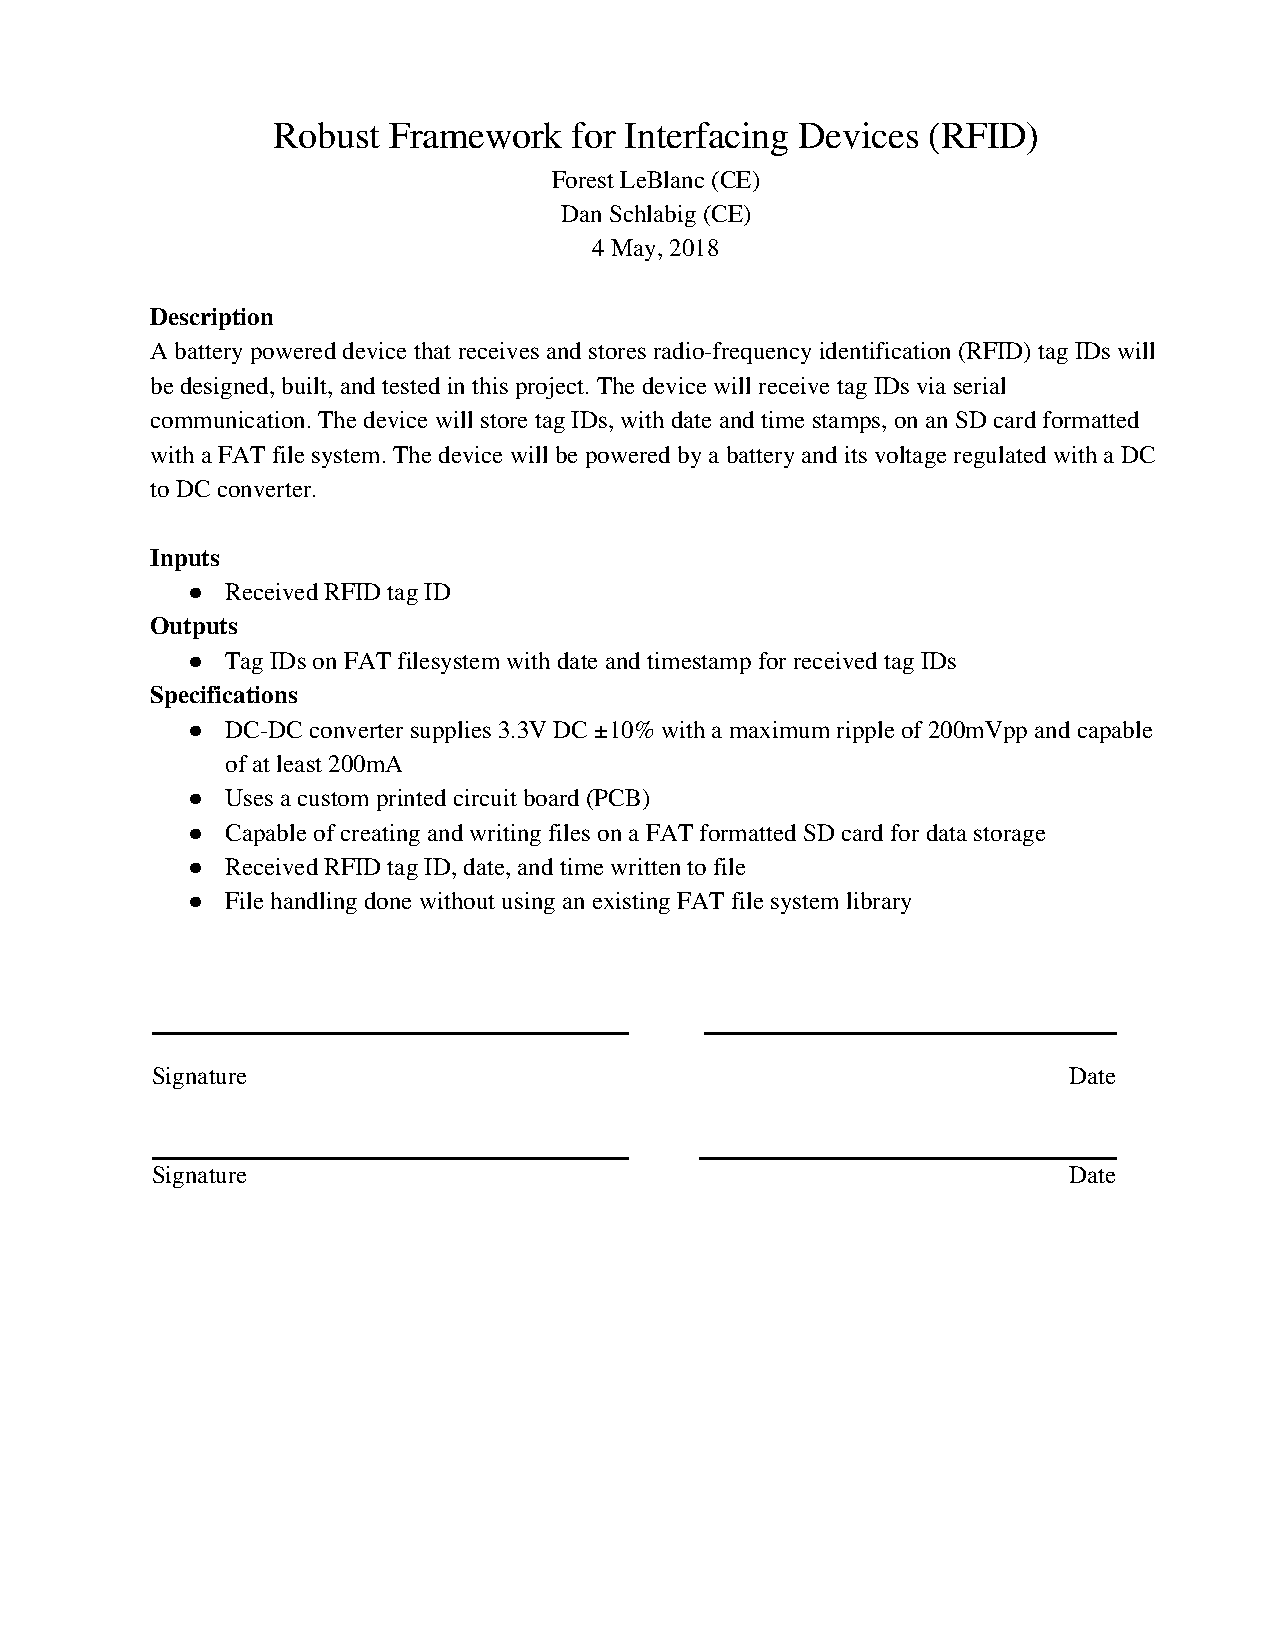
\includegraphics[width=\textwidth]{Figures/appendix/Contract.pdf}

%\endpage

\section{Schematics}
%\centering
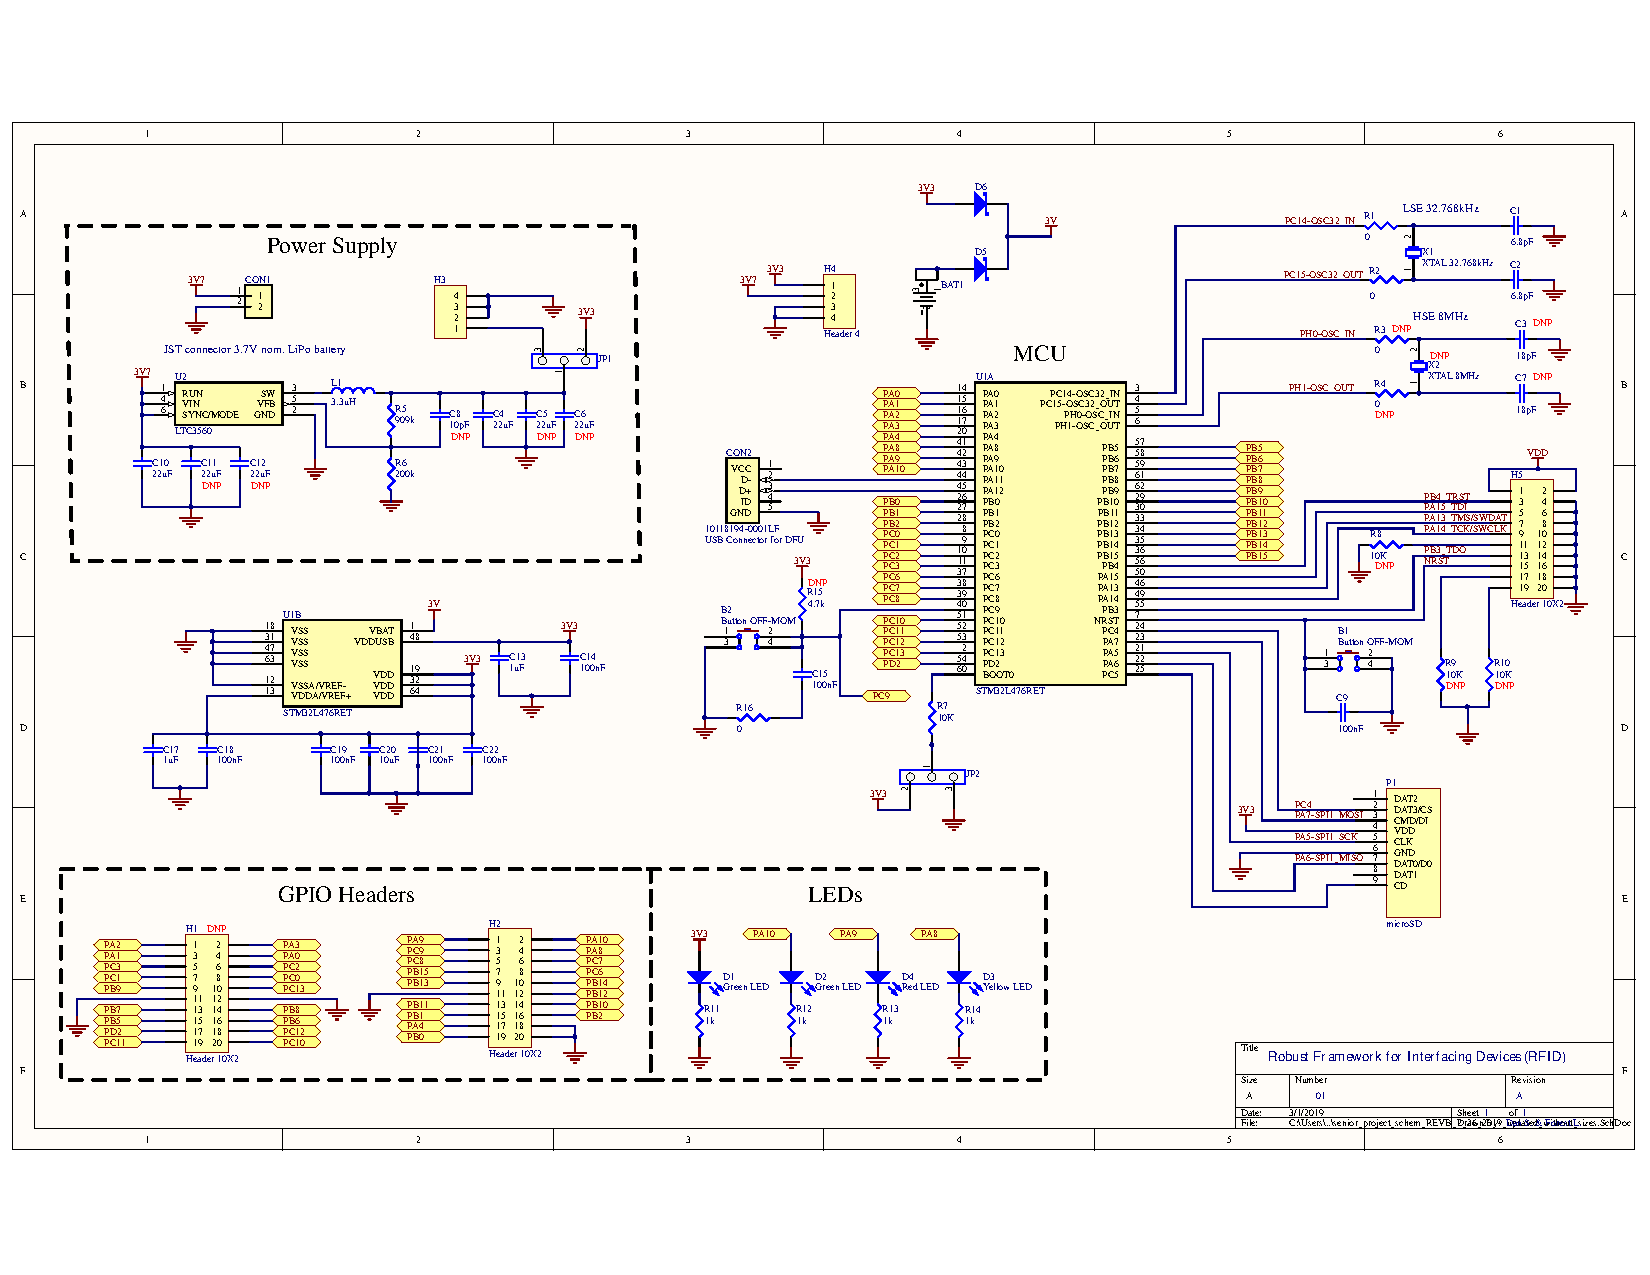
\includegraphics[scale=.75, angle=90]{Figures/appendix/senior_project_schem_REVB_3_1_2019_roughdraft.pdf}

\section{Parts List}

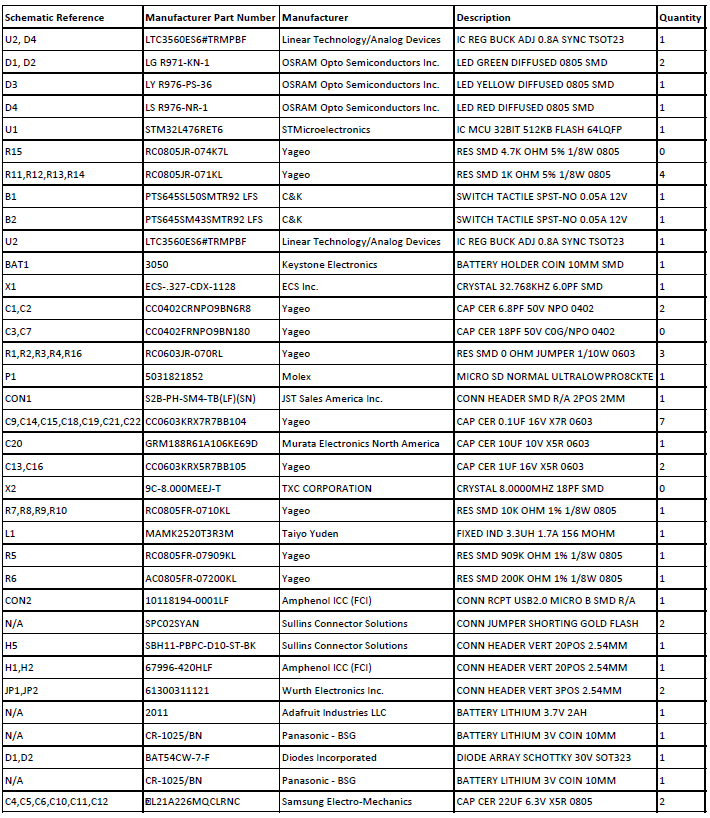
\includegraphics[width=\textwidth]{Figures/appendix/parts_list_3_1_2019_roughdraft.PNG}
%\endpage


%\section{Datasheets}

%\section{Operating Instructions}


% COMMENT OUT TO EXCLUDE SOURCE CODE
%\pagenumbering{gobble}
%%%%%%%%%%%%%%%%%%%%%%%%%%%%%%%%
% code listings (just formatting for nice print, comment out as needed in main.tex)
%%%%%%%%%%%%%%%%%%%%%%%%%%%%%%%
\newcommand{\codeListing}[2]{
\subsection{\detokenize{#1}}
\label{#1}
\lstinputlisting[language=#2]{#1}
}

\codeListing{sourcecode/main.c}{C}

\codeListing{sourcecode/global_config.c}{C}
\codeListing{sourcecode/global_config.h}{C}

\codeListing{sourcecode/core.c}{C}
\codeListing{sourcecode/core.h}{C}

\codeListing{sourcecode/myFat_diskio.c}{C}
\codeListing{sourcecode/myFat_diskio.h}{C}

\codeListing{sourcecode/tag-generator.py}{Python}



\end{document}